\scanpage{78}
polyèdres dans complexe cubique $\Bigg\{$

prismes \hspace{2em} $45.16$
\figure{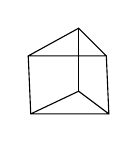
\begin{tikzpicture}[x=.032cm,y=-.032cm,line cap=round,line join=round]
\draw (0,11) -- (31,11) -- (20,0) -- cycle;
\draw (1,34) -- (32,34) -- (20,25) -- cycle;
\draw (0,11) -- (1,34);
\draw (31,11) -- (32,34);
\draw (20,0) -- (20,25);


\end{tikzpicture}}
prismes doubles \hspace{2em} $45.8$
\figure{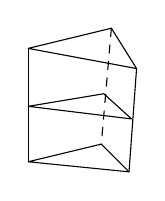
\begin{tikzpicture}[x=.032cm,y=-.032cm,line cap=round,line join=round]
\draw (0,8) -- (43,16) -- (33,0) -- cycle;
\draw (0,31) -- (41,36) -- (30,26) -- cycle;
\draw (0,53) -- (40,57) -- (29,46) -- cycle;
\draw (0,8) -- (0,53);
\draw (43,16) -- (40,57);
\draw[dashed] (33,0) -- (29,46);


\end{tikzpicture}}
antiprisme \unsure{torseur|torseur tordu|tordus} (\deleted{\unsure{appa|app|appelons}} \unsure{plan} projectif réel)
\margin{avec grain de sel pour le disque (faux) hexagonal qui \unsure{transforme|ferme} le \unsure{bandeau|ruban} de Möbius}
% slanted
\figure{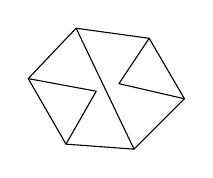
\begin{tikzpicture}[x=.032cm,y=-.032cm,line cap=round,line join=round]
\draw (0,20) -- (19,0) -- (48,4) -- (62,28) -- (42,48) -- (15,46) -- cycle;
\draw (19,0) -- (42,48);
\draw (0,20) -- (27,25) -- (15,46);
\draw (48,4) -- (36,22) -- (62,28);


\end{tikzpicture}}
pseudocube (cube avec $1$ arête contractée) \hspace{1em} $45.\deleted{\unsure{8|9}}.16.3=2^4 3^4 5$
\figure{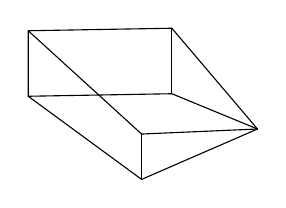
\begin{tikzpicture}[x=.032cm,y=-.032cm,line cap=round,line join=round]
\draw (0,1) -- (57,0) -- (91,40) -- (45,60) -- (0,27) -- cycle;
\draw (0,1) -- (45,42) -- (91,40);
\draw (45,42) -- (45,60);
\draw (0,27) -- (57,26) -- (91,40);
\draw (57,0) -- (57,26);


\end{tikzpicture}}
\uline{cubes} \hspace{1em} $27.10.\deleted{\unsure{4|1}}2=2^2.3^3.5$

dodécaèdre gauche \hspace{1em} $2^4.3^3=36.12=36.6.2$.

\diagram{\(\text{polygones}\quad\left\{\begin{array}{ll}
\text{carrés}&27.10.4=2^3 3^3 5\\
\text{pentagones}&36.6.12=2^5.3^4\\
\text{hexagones}&720=2^4.3^2.5
\end{array}\right.\)}

\figure{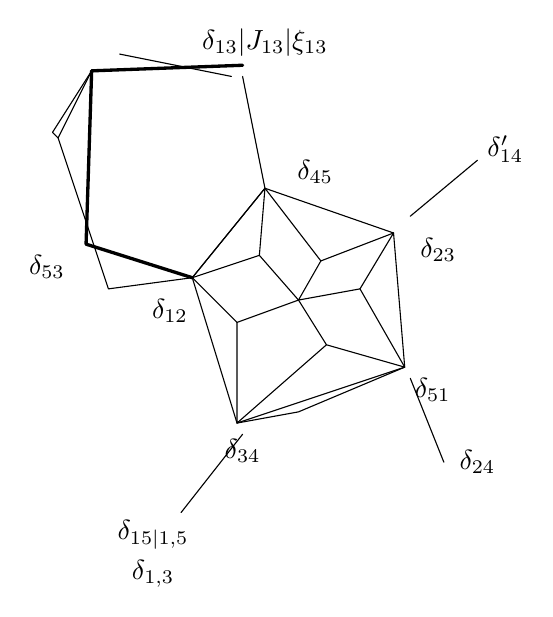
\begin{tikzpicture}[x=.071cm,y=-.071cm,line cap=round,line join=round]
\draw[very thick] (13,9) -- (40,8);
\draw[very thick] (13,9) -- (12,40) -- (31,46);
\draw (40,10) -- (44,30) -- (31,46) -- (16,48) -- (7,21) -- (13,9);
\draw (13,9) -- (6,20) -- (7,21);
\draw (18,6) -- (38,10);
\draw (44,30) -- (67,38) -- (69,62) -- (50,70) -- (39,72) -- (31,46) -- (44,30);
\draw (31,46) -- (43,42) -- (44,30);
\draw (43,42) -- (50,50) -- (39,54) -- (31,46);
\draw (39,54) -- (39,72) -- (55,58) -- (50,50);
\draw (44,30) -- (54,43) -- (67,38);
\draw (54,43) -- (50,50) -- (61,48) -- (67,38);
\draw (61,48) -- (69,62) -- (55,58);
\draw (69,62) -- (39,72);
\draw (70,35) -- (82,25);
\draw (40,74) -- (29,88);
\draw (70,64) -- (76,79);
\node[inner sep=.5pt] at (44,4) {$\unsure{\delta_{13}|J_{13}|\xi_{13}}$};
\node[inner sep=.5pt] at (53,27) {$\delta_{45}$};
\node[inner sep=.5pt] at (5,44) {$\delta_{53}$};
\node[inner sep=.5pt] at (27,52) {$\delta_{12}$};
\node[inner sep=.5pt] at (87,23) {$\delta'_{14}$};
\node[inner sep=.5pt] at (75,41) {$\delta_{23}$};
\node[inner sep=.5pt] at (74,66) {$\delta_{51}$};
\node[inner sep=.5pt] at (82,79) {$\delta_{24}$};
\node[inner sep=.5pt] at (40,77) {$\delta_{34}$};
\node[inner sep=.5pt] at (24,92) {$\delta_{\unsure{15|1,5}}$};
\node[inner sep=.5pt] at (24,99) {$\delta_{1,3}$};

\end{tikzpicture}}
$\underline{1\ 2\ 3\ 4\ \underline{5}}$
\figure{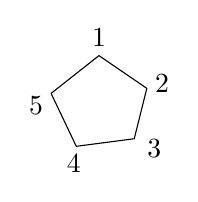
\begin{tikzpicture}[x=.032cm,y=-.032cm,line cap=round,line join=round]
\draw (4,16) -- (23,1) -- (42,14) -- (37,34) -- (14,37) -- cycle;
\node[inner sep=.5pt] at (23,-6) {$1$};
\node[inner sep=.5pt] at (48,12) {$2$};
\node[inner sep=.5pt] at (45,38) {$3$};
\node[inner sep=.5pt] at (13,44) {$4$};
\node[inner sep=.5pt] at (-2,21) {$5$};

\end{tikzpicture}}
\figure{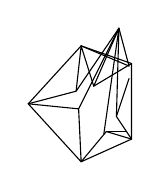
\begin{tikzpicture}[x=.032cm,y=-.032cm,line cap=round,line join=round]
\draw (0,30) -- (21,7) -- (41,14) -- (41,44) -- (21,53) -- cycle;
\draw (0,30) -- (19,25) -- (21,7) -- (26,23) -- (41,14);
\draw (0,30) -- (20,32) -- (21,53) -- (31,41) -- (41,44);
\draw (20,32) -- (36,0) -- (30,42);
\draw (19,25) -- (36,0) -- (35,35) -- (41,44);
\draw (26,23) -- (36,0) -- (40,15);
\draw (21,7) -- (40,15);
\draw (31,41) -- (39,41);
\draw (35,35) -- (40,20);


\end{tikzpicture}}
\figure{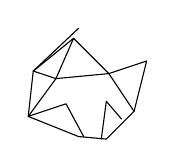
\begin{tikzpicture}[x=.032cm,y=-.032cm,line cap=round,line join=round]
\draw (2,17) -- (18,4) -- (32,18) -- (47,13) -- (42,33) -- (31,44) -- (20,43) -- (0,35) -- cycle;
\draw (2,17) -- (11,20) -- (18,4);
\draw (11,20) -- (0,35) -- (15,30) -- (22,43);
\draw (11,20) -- (32,18) -- (42,33);
\draw (29,44) -- (31,29) -- (37,36);
\draw (2,17) -- (20,0);


\end{tikzpicture}}
\figure{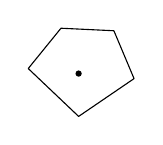
\begin{tikzpicture}[x=.032cm,y=-.032cm,line cap=round,line join=round]
\draw (0,16) -- (13,0) -- (34,1) -- (42,20) -- (20,35) -- cycle;

\fill (20,18) circle (.04cm);
\end{tikzpicture}}
$\delta_{56}\ \delta_{26}.\delta_{46}\ \delta_{16}\ \delta_{36}$
\[
\left|\begin{matrix}\delta_6\\\delta'_6\end{matrix}\right.\qquad
\deleted{\delta_{\unsure{123|23}}}\ 
\underbrace{\delta_{12}\ \delta_{34}\ \delta_{51}\ \delta_{23}}_{\text{pentagones}}\ \delta_{45}
\qquad 5.2\qquad 4!/2=
\]
\[
\begin{aligned}
2^5.3^4&=36.6.12\\
2^{8}\unsure{4|.}.5&\quad\text{\uline{aut.}}
\end{aligned}
\]

% The following block is upside down on the sheet and has long diagonal cancellation strokes.
\deleted{
\diagram{\(\begin{array}{rll}
 &C&I\amalg I\amalg\unsure{\mathfrak P_2|\mathscr P_2}(I)\\
 &&\delta_i\qquad\delta'_i\qquad\delta_{ij}\\
27\mid&\mathbb Z[C]&c.c'=\begin{cases}-1&\text{si }c=c'\\0&\text{si }c\ne c'\quad c,c'\text{ non liés}\\1&\text{si }c\ne c',\quad c',c''\text{ liés}\end{cases}\\
 &\downarrow&\\
7&\widehat E(C)&\underbrace{\delta_1,--\delta_6\quad\unsure{\eta|y}}_{\lambda.\deleted{\unsure{\delta|z|\sum}}\delta=1}=\delta_{ij}+\delta_i+\delta_j\qquad i\ne j\\
 &\rotatebox{90}{$\ni$}&\\
 &\lambda&\\
6&E(C)=\lambda^\perp&\\
 &\multicolumn{2}{l}{\{\delta'-\delta\mid\delta,\delta'\in C,\quad\delta,\delta'\text{ non liés}\}}\\
72&&\dfrac{\overset{\frown}{27.16}}6=72
\end{array}\)}
\figure{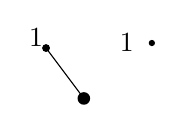
\begin{tikzpicture}[x=.032cm,y=-.032cm,line cap=round,line join=round]
\draw (4,5) -- (19,25);
\node[inner sep=.5pt] at (0,1) {$1$};
\node[inner sep=.5pt] at (36,3) {$1$};
\fill (4,5) circle (.05cm) (19,25) circle (.08cm) (46,3) circle (.04cm);
\end{tikzpicture}}
\[
\deleted{\begin{aligned}
&\sum_{b\in\unsure{\mathrm{Bas}|\mathrm{Bases}}(C)}\ \sum_{\beta\in\unsure{\mathcal P_{2,2,2}|\mathfrak P_{2,2,2}}(b)}\pi(\beta)\\
& b=\{\underbrace{b_1,\ },\underbrace{\ --\ },\underbrace{b_6}\}
\end{aligned}}
\]
\[
\begin{aligned}
b&=\{(b_i)_{1\leq i\unsure{\in|\leq}6}\} &\underbrace{b'_i-b_i}&=r_b\\
b'&=\{(b'_i)_{1\leq i\leq6}\}
\end{aligned}
\]
}
% archive sheet number: 77
